% --
% Neural Network Architectures

\chapter{Neural Networks}\label{sec:nn}
%This chapter contains theoretical foundations and practical evaluation of developing a Key Word Spotting (KWS) system with neural networks, especially intended for video games
This chapter contains theoretical foundations and details about the used neural networks architectures applied to Key Word Spotting (KWS) of speech commands.
The training of the used neural networks and some special concepts, such as adversarial pre-training, are presented and experimental results shown.
Special focus is lied on energy efficiency and therefore each networks energy footprint is evaluated.


% theory
% --
% theory

\section{Theory}\label{sec:nn_theory}
\thesisStateNotReady
The theory provided in this sections merely focuses on the used neural network architectures and some basic theory elements in neural networks.
The most basic element in neural networks is described here as node, an abstract element, usually illustrated as circle, that defines input and output connections from and to other nodes within the network.
The connections from and to a node are multiplications with scalar values, denoted as weight.
Each node usually incorporates an additive term, denoted as bias term.
All weights and bias terms are forming the parameters of a network and can be trained through back-propagation.
The output of a node is a scalar computed from all inputs and mapped with a non-linear function denoted as activation function.
A neural network can consist of thousand of nodes in each possible constellation of connections.
In this thesis, the focus is only on single directional connections (no bidirectional connections).
The structure of a neural network is defined by its layers, where a layer is a set of nodes with specific connection properties that receive inputs from the previous layer and output connections to the next layer.
For example, a neural network consists one convolutional layer followed by three fully connected layers.
The last layer of a neural network represents for instance the class labels of a classification tasks.
A loss function computes the difference between the predicted and the actual class label during training and is essential for the backpropagation algorithm that updates each parameter in the network through the gradients of the obtained error.


% --
% activation functions

\subsection{Activation Functions}\label{sec:nn_theory_acti}
Activation functions for neural networks of a node in a current layer are non-linear functions that usually maps the sum of the weighted inputs from nodes in a previous layer to a single output value $z$ as following:
\begin{equation}\label{eq:nn_theory_acti}
  z = h(w \, x^T)
\end{equation}
where $h$ is the activation function, $w \in \R^n$ is an weight vector and $x \in \R^n$ an input vector for one specific node.
The output of each node in a current layer is further connected to other nodes in the next layer and builds up the neural network.
The constraint of an activation function is, that an easy computable derivative of this function exist, in order to backpropagate gradients.

The most famous activation function nowadays is the RELU function:
\begin{equation}\label{eq:nn_theory_relu}
  z = \max{(0, a)}
\end{equation}
with $a \in \R$ as input to the activation function.
The big advantage is that this function and its subgradients are very easy and fast to compute.
The two other activation functions that are used in wavenets are the sigmoid function:
\begin{equation}\label{eq:nn_theory_sigmoid}
  z = \frac{1}{1 + \exp{-x}}
\end{equation}
and the tanh functions:
\begin{equation}\label{eq:nn_theory_tanh}
  z = \frac{\exp{x} - \exp{-x}}{\exp{x} + \exp{-x}}
\end{equation}


% --
% fully connected

\subsection{Fully Connected Layer}
A fully connected (FC) layer is the simplest layer type in neural networks.
Each node from the previous layer is connected in forward direction to all nodes in the FC layer and each node in the FC layer is further connected to all nodes in the next layer.
Further each connection has one trainable weight and each node has a bias term.
A simple FC layer is illustrated in \rfig{nn_theory_fc}.
% fc
\begin{figure}[!ht]
  \centering
    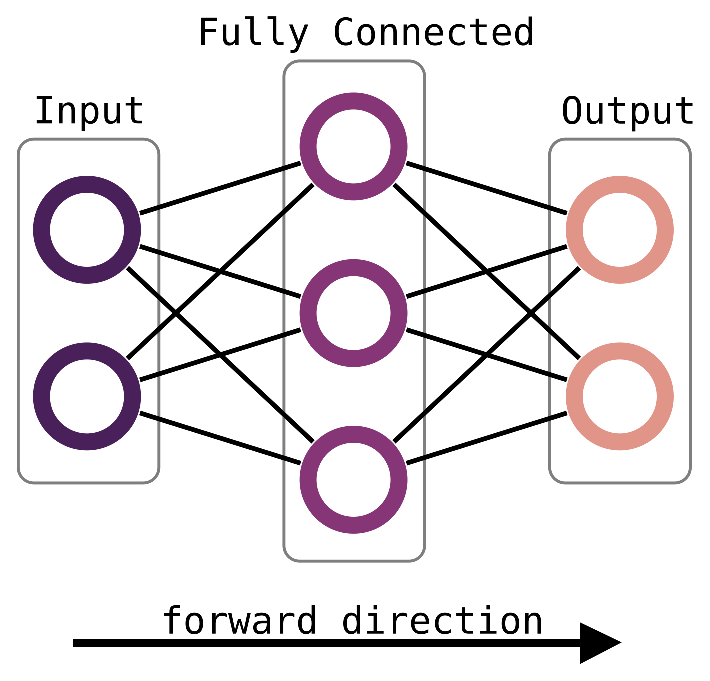
\includegraphics[width=0.30\textwidth]{./4_nn/figs/nn_theory_fc.eps}
  \caption{Basic fully connected layer with 3 nodes, receiving connections from 2 input nodes and outputing connections to 2 output nodes.}
  \label{fig:nn_theory_fc}
\end{figure}
\FloatBarrier
\noindent
In one node usually following computation is processed:
\begin{equation}
  z = h(w \, x^T + b)
\end{equation}
with the same notations as in \req{nn_theory_acti} and an additional bias term $b \in \R$.


% --
% cnn

\subsection{Convolutional Layers}\label{sec:nn_theory_cnn}
Convolutional layers are the fundament of every Covolutional Neural Networks (CNN) as already discussed in \rsec{prev_nn_cnn}.
They use convolutional filters on small areas of the input data, so that spatial information is retrieved.
Those convolutional filters are also called kernels and illustrated in case of images as rectangle in 2D space with kernel width $k_w$ and height $k_h$.
The kernel is shifted over its input map in each axis with an operation called \emph{stride}, denoted as $s$, and produce a output map through convolution.
The output dimension $o_d$ for striding along this axis with $s_d$ and kernel size for that axis $k_d$ over the input dimension $i_d$ can be computed as:
\begin{equation}\label{eq:nn_theory_cnn_}
  o_d = \floor*{\frac{i_d + p_d - k_d}{s_d} + 1}
\end{equation}
where $p_d$ is additionally a \emph{padding} term, where for instance for in zero-padding, zeros are added on both sides of the input dimension.
For example if a $16 \times 16$ image is convoluted by a $5 \times 5$ kernel with stride $1$ in each direction and no padding, the output image is $12 \times 12$.
The padding operation has usually the purpose to keep a the output and input dimension the same.
This is used for instance in residual neural networks, where the input to convolutional layers of a block, is bypassed and added to the output of this block again.
Being able to compute the addition operation from input and output of the residual block, their dimensions must be the same.
However in most convolutional network applications without residual blocks, it is preferred not to pad the image, so that dimensions are reduced hence parameters and multiplications saved.
Further there exist some special convolutional layers designed to reduce the dimensions (subsampling), such as a Max-Pooling layer. 

As already mentioned above CNNs are defined with the amount of input and output channels (feature maps), the kernel size, the stride of the kernel and some other specialties like dilation.
However it is not immediately clear from those parameter, how many convolutional filters are applied and what how the output feature maps are calculated exactly.
The amount of convolutional filters is in most practical examples always:
\begin{equation}\label{eq:nn_theory_n_filters}
  \#k = i \cdot j
\end{equation}
where $i$ and $j$ is the amount of input and output channels respectively.
Each kernel produces an output map, but the idea is to constraint the number of output maps $\#k$ to the defined output channels $j$.
This is usually done by summing up all output maps of input channels $i$ for one output channel $j$:
\begin{equation}
  o_j = \sum_{i} k_{i, j} * x_i
\end{equation}
where $o_j$ is the j-th feature map, $k_{i, j}$ the kernel of $i$ and $j$ and $x_i$ the i-th input channel.
A gaphical example of this procedure is shown in \rfig{nn_theory_cnn_basics}.
% cnn basics
\begin{figure}[!ht]
  \centering
    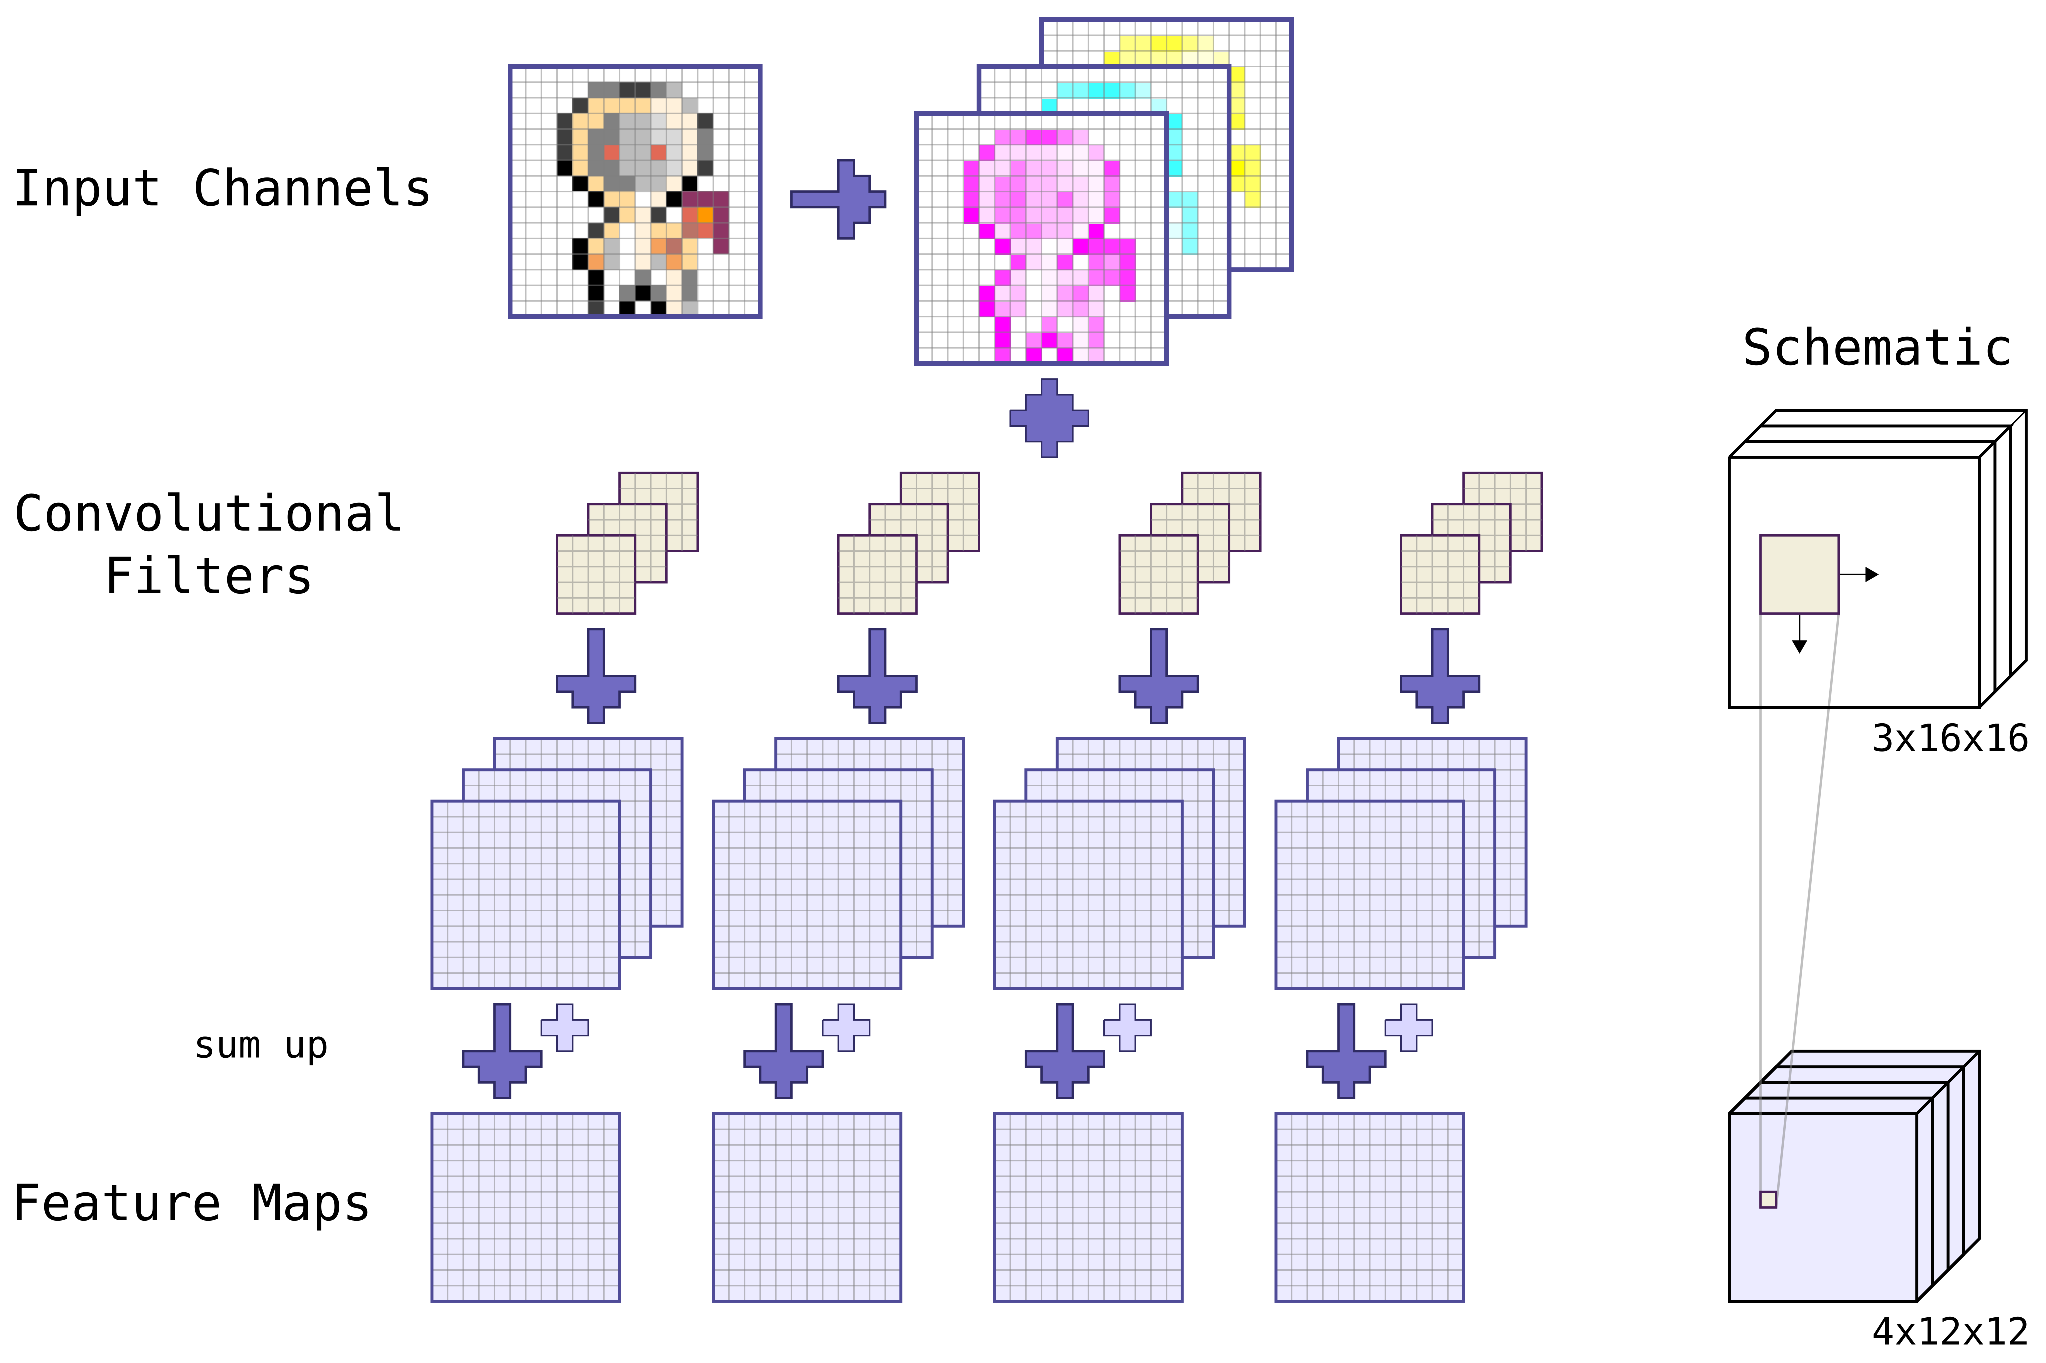
\includegraphics[width=0.6\textwidth]{./4_nn/figs/nn_theory_cnn_basics.eps}
  \caption{Basic CNN layer with a $16 \times 16$ input image, decomposed in 3 channels (CYM) and 4 output feature maps. Kernel size is $5 \times 5$ and the stride is $1$.}
  \label{fig:nn_theory_cnn_basics}
\end{figure}
\FloatBarrier
\noindent


% --
% loss functions

\subsection{Loss Functions and Softmax}
Loss functions or also called cost functions are used to calculate the difference between the predicted labels $\hat{y}$ compared to the actual or ground truth labels $y$.
The predicted labels are usually presented by the output nodes in the last layer of a neural network.
Therefore $\hat{y} = [\hat{y_1}, \, \hat{y_2}, \dots, \hat{y_c}]^T$ has the dimension of the number of labels or classes $c$.
Often it is preferred that $\hat{y} \in R^c$ provides a probability distribution such that:
\begin{equation}
  \sum_{i=0}^c \hat{y}_i = 1
\end{equation}
which can be achieved with the softmax function:
\begin{equation}\label{eq:nn_theory_softmax}
  \hat{y}_i = \frac{\exp{x_i}}{\sum_{j=0}^{c}\exp{x_j}}
\end{equation}
where $c$ is the amount of nodes in this layer, if it is the last layer as usual for the softmax, $c$ is the amount of classes and $\hat{y}_i$ the probability value of the corresponding class $i$.


% --
% dropout

\subsection{Dropout}
Dropout is a method to improve generalization and training of neural network.
The idea is to set the output of randomly selected nodes within a layer and for one training step to zero, so that only the other nodes are updated.
This can be simply done by multiplying all outputs of a current layer with a vector containing a number of zeros and ones places at random positions within the vector.
The amount of zeros compared to ones can be determined by a probability value, for instance $p=0.2$ means that there are 20\% zeros and 80\% ones within the vector.


% --
% training

\subsection{Training of a Neural Network}
The training process of a neural network is usually done with backpropagation of gradients from a loss function at the output nodes.
The backpropagation algorithm is not described here, because there exists many books and papers such as ... with good formulations, further it does not add any value to this thesis as the algorithm is run in the background of all neural network frameworks.
The interesting elements are therefore only the neural network architecture and the loss functions.


% architectures
% --
% Neural Network Architectures

\section{Neural Network Architectures}\label{sec:nn_arch}
All neural network Architectures evaluated within this thesis are presented here.
In general the used architectures were:
\begin{enumerate}
	\item Convolutional Neural Networks (CNN)
	\item Generative Adversarial Neural Networks (GAN)
	\item Wavenets
\end{enumerate}
The term convolutional neural network here consists of all architectures consisting of at least one convolutional layer and the intention to simply classify each speech commands from each other. 
Therefore the output of a convolutional net is of size of the number of individual speech commands and usually has some kind of probability distribution or energy equivalence.

With adversarial neural networks all architectures are meant, with at least two separate neural network Architectures, e.g. a Discriminator and a Generator Network and the intention to outperform the other Network in a task where both play a game against each other.
The word game is meant in the sense of game theory, where the goal is to find an equilibrium state of players competing against each other.
An equilibrium state is usually found if all players are satisfied with the outcome.
In this thesis the amount of players, or neural networks, is always two.
An overview of all models is shown in \rtab{nn_arch_overview} with abbreviations in \rtab{nn_arch_abbreviation}.
\begin{table}[ht!]
\small
\begin{center}
\caption{Network Architectures Abbreviations}
\begin{tabular}{ M{2.5cm}  M{10cm} }
\toprule
\textbf{Abbreviations} & \textbf{Meaning}\\
\midrule
c[0-9] & convolutional layer with layer number\\
f[0-9] & feed forward fully-connected layer with layer number\\
m[0-9] & max pooling layer layer with layer number\\
ch & input channel number for mfccs it is usually 1\\
fs & frame size (usually 50 -> 50ms)\\
ms & feature size (mfcc), depends on feature selection\\
cf & output number of last flattened convolutional layer\\
cl & number of class labels\\
\bottomrule
\label{tab:nn_arch_abbreviation}
\end{tabular}
\end{center}
\vspace{-4mm}
\end{table}
\FloatBarrier
\noindent
\begin{table}[ht!]
\begin{center}
\caption{Network Architectures Overview with reference names}
\begin{tabular}{ M{2.5cm}  M{2.1cm}  M{2.1cm} M{2.1cm} M{2.5cm}}
\toprule
%\multicolumn{4}{c}{\textbf{Feature Groups}} & \multicolumn{2}{c}{\textbf{Accuracy}} \\
\textbf{Reference name} & \textbf{Feature maps} & \textbf{Kernel sizes} & \textbf{Strides} & \textbf{Feed Forward} \\
\midrule
conv-trad & c1: (ch, 64) c2: (64, 64) & c1: (4, 20) mp: (2, 4) c2: (2, 4) & c1: (1, 1) mp: (2, 4) c2: (1, 1) & f1: (cf, 32) \quad f2: (32, 128) f3: (128, cl)\\
\midrule
conv-fstride & c1: (ch, 54) & c1: (8, fs) & c1: (4, 1) & f1: (cf, 32) \quad f2: (32, 128) \quad f3: (128, 128) \quad f4: (128, cl)\\
\midrule
conv-encoder-fc1 & c1: (ch, 48) \quad c2: (48, 8) & c1: (ms, 20) \quad c2: (1, 5) & c1: (1, 1) \quad c2: (1, 1) & f1: (cf, cl)\\
\midrule
conv-encoder-fc3 & c1: (ch, 48) \quad c2: (48, 8) & c1: (ms, 20) \quad c2: (1, 5) & c1: (1, 1) \quad c2: (1, 1) & f1: (cf, 64) \quad f2: (64, 32) \quad f3: (32, l)\\
\bottomrule
\label{tab:nn_arch_overview}
\end{tabular}
\end{center}
\end{table}
\FloatBarrier
\noindent



% adversarial
% --
% adversarial

\section{Adversarial Pre-Training}\label{sec:nn_adv}
\thesisStateRevised
In adversarial neural network training, two separate neural networks are competing against each other in an adversary task.
This competition of the two networks motivates them to improve their performance and beat the other network.
The application of GANs, as already explained in \rsec{prev_nn_adv} and \rsec{nn_theory_gan}, is an interesting subject in research and the questions whether the obtained weights from the training of the Generator (G) and Discriminator (D) network can contribute to better the performances in equivalent models, arises.
In the following the training algorithms are explained in more detail, such as the loss functions used for G and D.
The transfer of weights can be done for training instances on small subsets of labels or the whole network by regarding all labels at once in a single training instance.
%The transferring technique of the whole network is denoted as adversarial dual train and the training of separate labels is named adversarial label train.
The transferring technique of training instances on small subsets of labels is denoted as adversarial label train and the transfer of weights from a whole network with all labels is named as adversarial dual train.
In the following those training techniques are further explained, except of the adversarial dual train, because it is straight forward if the adversarial label train is explained.

% --
% training GANs

\subsection{Training Generative Adversarial Neural Networks}
The interesting part in training GANs is how the Generator (G) and Discriminator (D) models are updated in each training step and which loss functions were used.
In \req{nn_theory_gan} the game is notated as min-max game, from which the loss of D $l_D$ can be described for one specific training example $i$ of a batch as:
\begin{equation}
  l_D(x_i, z_i, G) = l(D(x_i), y_r) + l(D(G(z_i)), y_f)
\end{equation}
where $l$ is the binary cross-entropy loss described in \req{nn_theory_binary_cross_entropy}, $D: \mathcal{X} \mapsto [0, 1]$ and $G: \mathcal{Z} \mapsto \mathcal{X}$, $x_i \in \mathcal{X}$ is the data example, $z_i \in \mathcal{Z}$ is a randomly sampled latent variable, $y_r = 1$ is the real label and $y_f = 0$ the fake label for that specific example $i$.
In contrast the loss of the Generators $l_G$ is:
\begin{equation}
  l_G(z_i, D) =  l(D(G(z_i)), y_r)
\end{equation}
with $y_r$ as real label to perform maximization of $\log D(G(\bm{z}))$ as described in \rsec{nn_theory_gan}.
An extended approach, so that G produces samples specifically similar to the data distribution and does not drift off into creating unrealistic fakes of noisy samples to fake D, is to incorporate a similarity term with the \emph{cosine similarity}:
\begin{equation}
  s(\bm{x_1}, \bm{x_2}) = \frac{\bm{x_1}^T \bm{x_2}}{\norm{\bm{x_1}}_2 \cdot \norm{\bm{x_2}}_2 + \epsilon} 
\end{equation}
where $s : (\mathcal{X}, \mathcal{X}) \mapsto [0, 1]$ is the cosine similarity function, $\bm{x_1}$ and $\bm{x_2}$ are two vectors for similarity measure and $\epsilon$ is a small number, such that no division by zero is possible.
With the similarity loss incorporated, $l_G$ gets:
\begin{equation}
  %l_G(x_i, z_i, D) =  l(D(G(z_i)), y_r) + \lambda (1 - \E \left[ s(x_i \bm{e}, G(z_i)) \right])
  l_G(x_i, z_i, D) =  l(D(G(z_i)), y_r) + \lambda \left(1 - \frac{1}{C} \sum_{c=0}^{C} s(\hat{\bm{e}}_c^T x_i , \hat{\bm{e}}_c^T G(z_i)) \right)
\end{equation}
where $\hat{\bm{e}}_c \in \{1, 0\}^C$ is a unit vector representing one cepstral coefficient of the Mel Frequency Cepstral Coefficient (MFCC) data $x_i \in \mathcal{X} = \R^{C \times M}$ with a total number of $C$ MFCC coefficients and $M$ frames.
Further $\lambda$ is a trade-off factor between data similarity and fake loss from D.
For the experiments in \rsec{exp_adv}, $\lambda = 5$ was chosen.

The update of D and G can be done for each training step by backpropagating the obtained losses.
However it is more appealing if D is updated for a certain numbers of training steps with no update of G and then alternating to updates of G without updating D.
This will give either D or G some update steps to improve in their specific adversarial task of either discriminating or generating.
In this thesis the training steps for updating either D or G was selected to 2 epochs.
Note that an epoch consists of several training steps depending on the batch size and amount of data, this can vary for the experiments, however it does not influence that much on the overall end results.


% --
% label train

\subsection{Adversarial Label Train}
Adversarial label train, is the transfer of weights from feature maps trained on multiple GAN training instances on subsets of all labels.
For instance if the total amount of labels are \{\enquote{left}, \enquote{right}\} then an own training instance can focus on the label \enquote{left} and another on the label \enquote{right}.
It is important to assign a specific number of feature maps to each label train instance, for example each label train gets 8 feature maps of the first convolutional layers.
The label train scheme is illustrated in \rfig{nn_adv_label_scheme} and applies 6 label train instances, such as used for the experiments in \rsec{exp_adv}.
\begin{figure}[!ht]
  \centering
    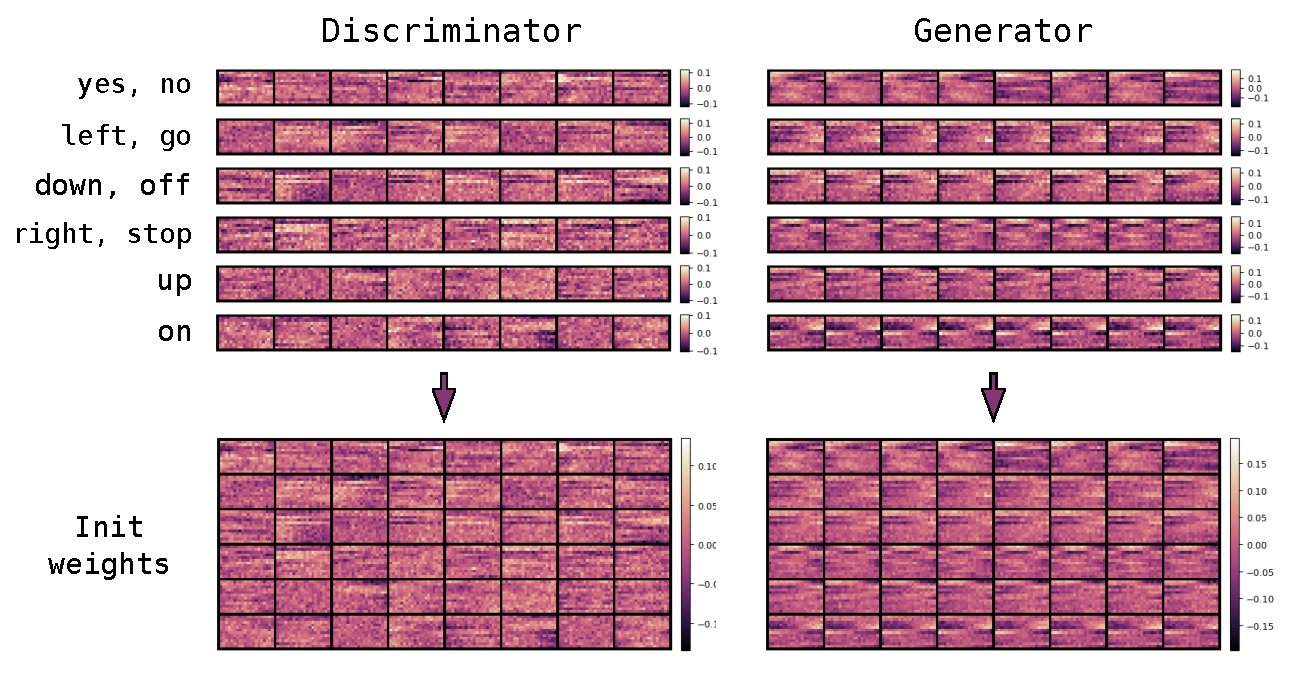
\includegraphics[width=0.7\textwidth]{./4_nn/figs/nn_adv_label_scheme}
  \caption{Label train scheme of 6 training instances, trained with 100 epochs for each label subset.}
  \label{fig:nn_adv_label_scheme}
\end{figure}
\FloatBarrier
\noindent
An actual GAN training for the labels \enquote{left} and \enquote{go} is shown in \rfig{nn_adv_loss_label}.
Note that the update of either the Discriminator (D) or Generator (G) model is done alternating for 2 training epochs.
\begin{figure}[!ht]
  \centering
  \subfigure[it-100]{\includegraphics[width=0.45\textwidth]{./4_nn/figs/nn_adv_loss_label_it-100}}
  \subfigure[it-1000]{\includegraphics[width=0.45\textwidth]{./4_nn/figs/nn_adv_loss_label_it-1000}}
  \caption{Adversarial training loss of the labels \enquote{left} and \enquote{go} with 8 feature maps.}
  \label{fig:nn_adv_loss_label}
\end{figure}
\FloatBarrier
\noindent
The creation of fake images from G is shown in \rfig{nn_adv_fakes_label} of the same training instances.
\begin{figure}[!ht]
  \centering
  \subfigure[it-100]{\includegraphics[width=0.45\textwidth]{./4_nn/figs/nn_adv_fakes_label_it-100}}
  \subfigure[it-1000]{\includegraphics[width=0.45\textwidth]{./4_nn/figs/nn_adv_fakes_label_it-1000}}
  \caption{Generation of fake images of the labels \enquote{left} and \enquote{go} with 8 feature maps for the GAN training.}
  \label{fig:nn_adv_fakes_label}
\end{figure}
\FloatBarrier
\noindent

As showcase example, some concatenated adversarial label train weights used for weight transfer, are shown for D and G with different amounts of training epochs in \rfig{nn_adv_label_weights_d} and \rfig{nn_adv_label_weights_g}.
\begin{figure}[!ht]
  \centering
  \subfigure[d-100]{\includegraphics[width=0.45\textwidth]{./4_nn/figs/nn_adv_label_weights_d-100}}
  \subfigure[d-1000]{\includegraphics[width=0.45\textwidth]{./4_nn/figs/nn_adv_label_weights_d-1000}}
  \caption{Concatenated label weights of the first convolutional layer from the Discriminator model with different amounts of epochs.}
  \label{fig:nn_adv_label_weights_d}
\end{figure}
\FloatBarrier
\noindent
\begin{figure}[!ht]
  \centering
  \subfigure[g-100]{\includegraphics[width=0.45\textwidth]{./4_nn/figs/nn_adv_label_weights_g-100}}
  \subfigure[g-1000]{\includegraphics[width=0.45\textwidth]{./4_nn/figs/nn_adv_label_weights_g-1000}}
  \caption{Concatenated label weights of the first convolutional layer from the Generator model with different amounts of epochs.}
  \label{fig:nn_adv_label_weights_g}
\end{figure}
\FloatBarrier
\noindent
The amounts of epochs are important, because they determine how much the models are learning in their adversarial task.
With 100 epochs the Generator creates similar feature maps for each label train instance, because it does not need to be that accurate in creating different looking fakes, however the Discriminator gets better as well and the need of generating different looking fakes are necessary to match up.
With 1000 epochs the Generator produces already different fakes as already shown in \rfig{nn_adv_fakes_label} however it is not recommended to train for too long.
Note that a second convolutional layer for the \texttt{adv-d-jim} and \texttt{adv-g-jim} exist as well, the corresponding weights are shown only for the 100 epoch examples in \rfig{nn_adv_label_weights_conv1}.
\begin{figure}[!ht]
  \centering
  \subfigure[d-100]{\includegraphics[width=0.25\textwidth]{./4_nn/figs/nn_adv_label_weights_conv1_d-100}}
  \qquad \qquad
  \subfigure[g-100]{\includegraphics[width=0.25\textwidth]{./4_nn/figs/nn_adv_label_weights_conv1_g-100}}
  \caption{Concatenated label weights of the second convolutional layer from the Discriminator and Generator model with trained with 100 epochs.}
  \label{fig:nn_adv_label_weights_conv1}
\end{figure}
\FloatBarrier
\noindent
From the second convolutional layer each row corresponds to a single feature map and therefore 8 rows to one adversarial label training instance.
% \subsection{Questions that arise}
% There are several questions that arise regarding Adversarial Training:
% \begin{enumerate}[label={Q.\textgoth{A}.\arabic*)}, leftmargin=1.4cm]
%   \item Does the Network Architecture of G and D have to be the same but transposed?
%   \item Does the value space of in and outputs, for D and G respectively, have to be limited between a range of [0, 1] done by for instance the frame normalization, or sigmoid output?
%   \item What loss function works well for training?
%   \item How long should be trained?
%   \item When transfering weights to another network, should the weights from G or D be transfered?
%   \item Does the classification network has to adapt the parameters from the transfered weights?
%   \item Whats the benefit of all this?
% \end{enumerate}

% To illustrate the idea an example is shown of the labels L5 (left, right, up, down, go).

% The convolutional layer weights from the adversarial training of the individual labels, 
% can be stacked together an used to initialize another network.
% An example of this method is shown in \rfig{nn_adv_example}, where the initialization pattern changes to more elaborate structures and patterns to form good classification outputs. 
% However the Basic Pattern from the adversarial training stays the same, which is a good sign, because then the network is accepting those trained weights and adapts them.

% \begin{figure}[!ht]
%   \centering
%     \subfigure[c1 trained]{\includegraphics[width=0.45\textwidth]{./4_nn/figs/nn_adv_example_c0}}
%     \subfigure[c1 init]{\includegraphics[width=0.45\textwidth]{./4_nn/figs/nn_adv_example_c0_init}}
%     \subfigure[c2 trained]{\includegraphics[height=0.45\textwidth]{./4_nn/figs/nn_adv_example_c1}}
%     \quad
%     \subfigure[c2 init]{\includegraphics[height=0.45\textwidth]{./4_nn/figs/nn_adv_example_c1_init}}
%   \caption{Adversarial Training Example: Convolutional layers pretrained with adversarial training on each label separately.}
%   \label{fig:nn_adv_example}
% \end{figure}
% \FloatBarrier
% \noindent

% For this example in adversarial training, 8 feature maps of the first layer were used for each label, also they belong to the Generator Network G or decoder (dec). In Convolutional Networks, each previous layers feature map creates a new set of feature maps in the next layer.
% An example of this label training is shown in \rfig{nn_adv_example_label} with feature maps [(1, 8), (8, 8)] of the convolutional layers

% \begin{figure}[!ht]
%   \centering
%     \subfigure[\enquote{left} c1 from D]{\includegraphics[width=0.45\textwidth]{./4_nn/figs/nn_adv_example_label_left_c0_enc}}
%     \subfigure[\enquote{left} c1 from G]{\includegraphics[width=0.45\textwidth]{./4_nn/figs/nn_adv_example_label_left_c0_dec}}
%     \subfigure[\enquote{left} c2 from D]{\includegraphics[width=0.3\textwidth]{./4_nn/figs/nn_adv_example_label_left_c1_enc}}
%     \subfigure[\enquote{left} c2 from G]{\includegraphics[width=0.3\textwidth]{./4_nn/figs/nn_adv_example_label_left_c1_dec}}
%   \caption{Adversarial Training example of Generator (G) and Discriminator (D) of label \enquote{left} captured with 8 feature maps of the first convolutional layer.}
%   \label{fig:nn_adv_example_label}
% \end{figure}
% \FloatBarrier
% \noindent

% Those trained weights from each label can then simply be put into the feature maps of a classification network.
% This is shown in \rfig{nn_adv_example} where c1 from G and c2 from G in \rfig{nn_adv_example_label} were transfered to the first row(s).
% When doing the transferring of feature maps, it is important that the layers are not mixed up so that the trained connections are still correct.
% Also of course the weights of the feature maps must have the same dimension, so that transferring is possible.


% \subsection{Observing the Generators output}
% While the output of the Discriminator is rather uninteresting (one-dimensional probability value), the output of the Generator is a good indicator of how well the training between D and G has gone.
% Optimally the output of the Generator look like real data samples.
% An example of a trained Generator Network with fake outputs compared to real ones is shown in \rfig{nn_adv_gen}.

% \begin{figure}[!ht]
%   \centering
%     \subfigure[\enquote{left} real examples]{\includegraphics[width=0.45\textwidth]{./4_nn/figs/nn_adv_gen_left_real}}
%     \subfigure[\enquote{left} fakes from G]{\includegraphics[width=0.45\textwidth]{./4_nn/figs/nn_adv_gen_left_fake}}
%   \caption{Real samples of \enquote{left} from the Speech Commands dataset compared to fake samples from a trained Generator Network.}
%   \label{fig:nn_adv_gen}
% \end{figure}
% \FloatBarrier
% \noindent

% If the fake example of the Generator Network do not look similar to real ones, then something might have gone wrong in the training between the Generator and Discriminator Network.
% Further it can be evaluated if a certain network architecture is able to produce a label in a sufficient representation, therefore this method might be a good start in finding a suitable network architecture for the problem to be solved.



